\documentclass[11pt,a4paper]{article}

% --- Packages ---
\usepackage[utf8]{inputenc}
\usepackage[T1]{fontenc}
\usepackage{amsmath,amssymb,amsfonts}
\usepackage{graphicx}
\usepackage{booktabs}
\usepackage{hyperref}
\usepackage[margin=1in]{geometry}
\usepackage{algorithm}
\usepackage{algpseudocode}
\usepackage{subcaption}
\usepackage{natbib}
\usepackage{xcolor}
\usepackage{float}
\usepackage{enumitem}

\hypersetup{colorlinks=true, linkcolor=blue, citecolor=blue, urlcolor=blue}

\title{Alpha-Graph: NLP-Driven Equity Signal Generation \\via SEC Filing Analysis and Machine Learning}
\author{Zhihan Lei}
\date{April 2026}

\begin{document}
\maketitle

\begin{abstract}
We present Alpha-Graph, a quantitative equity signal generation framework that extracts forward-looking information from SEC regulatory filings using a combination of natural language processing, large language model (LLM) agents, and gradient-boosted machine learning. The system ingests 10-K annual reports, 10-Q quarterly filings, and 8-K material event disclosures for 102 S\&P~500 constituents, generating cross-sectional return predictions via a walk-forward LightGBM combiner. Over a 24-month out-of-sample period (March~2024 to February~2026), the top-10/bottom-10 long/short portfolio achieves an annualized Sharpe ratio of \textbf{1.77}, cumulative return of \textbf{+80.5\%}, and maximum drawdown of \textbf{$-$13.3\%}, compared to $-$25.3\% and Sharpe $-$1.49 for the baseline Lazy Prices signal alone. The dominant predictive features are 8-K event scores and 21-day price momentum, confirming that high-frequency filing events contain material alpha beyond the annual filing change anomaly.
\end{abstract}

\section{Introduction}

Public companies in the United States are required to file periodic disclosures with the Securities and Exchange Commission (SEC). These filings---annual reports (10-K), quarterly reports (10-Q), and material event disclosures (8-K)---contain information about business operations, risk factors, litigation, management changes, and financial performance that is often overlooked by the market.

\citet{cohen2020lazy} documented the ``Lazy Prices'' anomaly: firms that substantially change the language of their annual filings subsequently underperform, suggesting that the market is slow to incorporate textual information from regulatory disclosures. While the original study relied exclusively on cosine similarity between consecutive 10-K filings, we extend this approach in three directions:

\begin{enumerate}[noitemsep]
    \item \textbf{8-K event-driven signals}: We score material events from 8-K filings by item type, providing signal updates multiple times per month rather than once per year.
    \item \textbf{Multi-agent LLM analysis}: We deploy specialized LLM agents (filing analyst, news synthesizer) to extract qualitative assessments of filing changes.
    \item \textbf{Machine learning signal combination}: We train a walk-forward LightGBM model to predict cross-sectional forward returns from heterogeneous signal features.
\end{enumerate}

\section{Data}

\subsection{SEC Filings}

We download filings from the SEC EDGAR database for 102 S\&P~500 constituents over a 3-year lookback period. Table~\ref{tab:filings} summarizes the dataset.

\begin{table}[H]
\centering
\caption{SEC filing dataset summary.}
\label{tab:filings}
\begin{tabular}{lrrr}
\toprule
Filing Type & Count & Avg.\ per Ticker & Description \\
\midrule
10-K & 401 & 3.9 & Annual report \\
10-Q & 935 & 9.2 & Quarterly report \\
8-K  & 4{,}146 & 40.6 & Material event disclosure \\
\midrule
\textbf{Total} & \textbf{5{,}482} & \textbf{53.7} & \\
\bottomrule
\end{tabular}
\end{table}

For 10-K and 10-Q filings, we extract three key sections: \emph{Item~1A---Risk Factors}, \emph{Item~7---Management's Discussion and Analysis} (MD\&A), and \emph{Item~1---Business Description}. For 8-K filings, we parse the item numbers from the filing metadata to identify the type of material event.

\subsection{Market Data}

We obtain daily OHLCV price data via Yahoo Finance for 94 tickers with complete coverage, spanning March~29, 2023 to March~27, 2026 (70{,}688 observations). Forward 21-trading-day returns serve as the prediction target. We compute rolling 21-day realized volatility, 5-day and 21-day momentum, and volume z-scores as auxiliary features.

\section{Signal Generation}

Our framework produces four categories of signals, summarized in Figure~\ref{fig:pipeline}.

\begin{figure}[H]
\centering
\fbox{\parbox{0.9\textwidth}{
\centering
\textbf{Signal Generation Pipeline} \\[6pt]
\begin{tabular}{ccccc}
10-K Filings & $\rightarrow$ & TF-IDF Cosine Similarity & $\rightarrow$ & Lazy Prices Score \\
8-K Filings & $\rightarrow$ & Item-Type Scoring & $\rightarrow$ & Event Score \\
Market Data & $\rightarrow$ & Gaussian HMM & $\rightarrow$ & Regime State \\
All Features & $\rightarrow$ & Walk-Forward LightGBM & $\rightarrow$ & \textbf{Predicted Return}
\end{tabular}
}}
\caption{Signal generation pipeline. Four signal sources are combined via a walk-forward LightGBM model.}
\label{fig:pipeline}
\end{figure}

\subsection{Lazy Prices: TF-IDF Cosine Similarity}
\label{sec:lazy}

Following \citet{cohen2020lazy}, we measure the textual similarity between consecutive 10-K filings for each company. For each filing pair $(d_{t-1}, d_t)$, we:

\begin{enumerate}[noitemsep]
    \item Tokenize and compute TF-IDF vectors with $n$-grams up to order 2, a vocabulary of 10{,}000 terms, and English stop-word removal.
    \item Compute cosine similarity:
    \begin{equation}
        \text{sim}(d_{t-1}, d_t) = \frac{\mathbf{v}_{t-1} \cdot \mathbf{v}_t}{\|\mathbf{v}_{t-1}\| \, \|\mathbf{v}_t\|}
    \end{equation}
\end{enumerate}

Across 299 filing pairs, the mean cosine similarity is $0.896$ (std $0.204$), with a minimum of $0.102$ (Altria Group, indicating a near-complete rewrite) and a maximum of $0.994$. We assign cross-sectional quintile ranks: the top quintile (highest similarity, least change) receives signal $+1$, and the bottom quintile receives signal $-1$.

\subsection{8-K Event-Driven Signal}
\label{sec:events}

The Lazy Prices signal updates only at 10-K filing frequency (approximately annual). To capture intra-year information, we introduce an 8-K event signal that updates whenever a company files a material event disclosure.

We assign a base score to each 8-K item type based on its expected impact on equity value:

\begin{table}[H]
\centering
\caption{8-K item scoring (selected items).}
\label{tab:8k_scores}
\begin{tabular}{llr}
\toprule
Item & Description & Score \\
\midrule
1.01 & Entry into material agreement & $+0.30$ \\
1.02 & Termination of material agreement & $-0.50$ \\
2.01 & Completion of acquisition/disposition & $+0.20$ \\
2.05 & Costs associated with exit/restructuring & $-0.40$ \\
4.01 & Changes in registrant's certifying accountant & $-0.70$ \\
5.02 & Departure of directors or principal officers & $-0.30$ \\
7.01 & Regulation FD disclosure & $0.00$ \\
\bottomrule
\end{tabular}
\end{table}

For each ticker, we compute an exponentially-weighted average of recent event scores with decay parameter $\lambda = 0.9$ per month:
\begin{equation}
    s_i = \frac{\sum_{k} w_k \cdot \text{score}(e_k)}{\sum_k w_k}, \quad w_k = \lambda^{\Delta t_k / 30}
\end{equation}
where $\Delta t_k$ is the number of days since event $e_k$. Across 102 tickers, the mean event score is $-0.005$ (std $0.062$), with 1{,}296 total 8-K events parsed.

\subsection{HMM Market Regime Detection}
\label{sec:regime}

We fit a 3-state Gaussian Hidden Markov Model to daily market features to classify the regime as \emph{Trending}, \emph{Mean-Reverting}, or \emph{Crisis}. Features include:

\begin{itemize}[noitemsep]
    \item 5-day rolling return of the S\&P~500 index
    \item 21-day rolling realized volatility
    \item Volatility ratio (5-day / 21-day)
\end{itemize}

All features are standardized prior to fitting. The HMM is estimated with full covariance matrices and 200 EM iterations. Regime labels are assigned post-hoc by volatility percentile of each state. Over the sample period, the market spent 76.1\% of days in the \emph{Trending} regime, 12.3\% in \emph{Mean-Reverting}, and 11.6\% in \emph{Crisis} (Table~\ref{tab:regimes}).

\begin{table}[H]
\centering
\caption{HMM regime distribution (731 trading days).}
\label{tab:regimes}
\begin{tabular}{lrr}
\toprule
Regime & Days & Fraction \\
\midrule
Trending & 556 & 76.1\% \\
Mean-Reverting & 90 & 12.3\% \\
Crisis & 85 & 11.6\% \\
\bottomrule
\end{tabular}
\end{table}

\subsection{Multi-Agent LLM Pipeline}

We deploy three specialized LLM agents (powered by DeepSeek-V3 via Together AI) in a fan-out/fan-in architecture built on LangGraph:

\begin{enumerate}[noitemsep]
    \item \textbf{Filing Analyst}: Compares current and previous 10-K filing text, identifies material changes in risk factors and MD\&A, and produces a signal in $[-1, +1]$ with a confidence score. The prompt explicitly asks for both risk assessment (negative signals) and opportunity detection (positive signals) to avoid bearish bias.
    \item \textbf{News Synthesizer}: Analyzes recent 8-K filings and categorizes events by materiality. Returns a signal and list of identified events.
    \item \textbf{Research Coordinator}: Combines agent signals using confidence-weighted averaging with an agreement penalty:
    \begin{equation}
        s_{\text{combined}} = \frac{\sum_i w_i \cdot c_i \cdot s_i}{\sum_i w_i \cdot c_i}, \quad c_{\text{final}} = \bar{c} \cdot (0.5 + 0.5 \cdot \text{agreement})
    \end{equation}
    where $w_i$ are agent weights, $c_i$ are confidence scores, and agreement measures directional consensus.
\end{enumerate}

\section{Machine Learning Signal Combination}
\label{sec:ml}

\subsection{Feature Panel}

We construct a daily cross-sectional panel of 94 tickers $\times$ 731 trading days (68{,}714 observations) with the following features:

\begin{table}[H]
\centering
\caption{ML combiner feature panel.}
\label{tab:features}
\begin{tabular}{llr}
\toprule
Feature & Source & Coverage \\
\midrule
\texttt{cosine\_similarity} & Lazy Prices (Section~\ref{sec:lazy}) & 66.1\% \\
\texttt{event\_score} & 8-K events (Section~\ref{sec:events}) & 100.0\% \\
\texttt{event\_count} & 8-K events & 100.0\% \\
\texttt{regime\_state} & HMM (Section~\ref{sec:regime}) & 97.1\% \\
\texttt{regime\_prob} & HMM posterior probability & 97.1\% \\
\texttt{momentum\_21d} & 21-day price return & 97.1\% \\
\texttt{momentum\_5d} & 5-day price return & 99.3\% \\
\texttt{volatility\_21d} & 21-day realized volatility & 97.1\% \\
\texttt{volume\_zscore} & Volume relative to 63-day average & 91.5\% \\
\bottomrule
\end{tabular}
\end{table}

Missing features are handled natively by LightGBM's NaN-aware split algorithm, avoiding the need for imputation.

\subsection{Walk-Forward Training}

To avoid lookahead bias, we train the model using a strict walk-forward protocol:

\begin{itemize}[noitemsep]
    \item \textbf{Training window}: 12 rolling months
    \item \textbf{Test window}: 1 calendar month
    \item \textbf{Purge gap}: 5 trading days between training end and test start
    \item \textbf{Target}: Forward 21-day return
    \item \textbf{Total folds}: 24 (March 2024 -- February 2026)
\end{itemize}

\subsection{Model Specification}

We use LightGBM \citep{ke2017lightgbm} with conservative hyperparameters designed to prevent overfitting:

\begin{table}[H]
\centering
\caption{LightGBM hyperparameters.}
\begin{tabular}{lr}
\toprule
Parameter & Value \\
\midrule
\texttt{num\_leaves} & 15 \\
\texttt{max\_depth} & 5 \\
\texttt{n\_estimators} & 200 \\
\texttt{learning\_rate} & 0.03 \\
\texttt{subsample} & 0.7 \\
\texttt{colsample\_bytree} & 0.7 \\
\texttt{reg\_alpha} (L1) & 0.1 \\
\texttt{reg\_lambda} (L2) & 1.0 \\
\texttt{min\_child\_samples} & 10 \\
\bottomrule
\end{tabular}
\end{table}

\subsection{Feature Importance}

Table~\ref{tab:importance} reports LightGBM split-based feature importance from the final trained model. The 8-K event score is the dominant feature, confirming that high-frequency filing events carry the strongest predictive signal.

\begin{table}[H]
\centering
\caption{Feature importance (split count) from final LightGBM model.}
\label{tab:importance}
\begin{tabular}{lr}
\toprule
Feature & Importance \\
\midrule
\texttt{event\_score} & 6 \\
\texttt{event\_count} & 3 \\
\texttt{momentum\_21d} & 2 \\
\texttt{regime\_state} & 1 \\
\texttt{momentum\_5d} & 1 \\
\texttt{volume\_zscore} & 1 \\
\texttt{cosine\_similarity} & 0 \\
\texttt{volatility\_21d} & 0 \\
\bottomrule
\end{tabular}
\end{table}

Notably, the Lazy Prices cosine similarity feature has zero importance in the final model, suggesting that the 8-K event signal subsumes the information content of annual filing changes when both are available.

\section{Portfolio Construction}

We construct a monthly-rebalanced long/short equity portfolio:

\begin{enumerate}[noitemsep]
    \item Rank all tickers by the ML combiner's predicted return signal.
    \item Go long the top 10 tickers (equal-weighted, 10\% each).
    \item Go short the bottom 10 tickers (equal-weighted, 10\% each).
    \item Apply transaction costs of 20 basis points per rebalance (conservative estimate for S\&P~500 constituents).
\end{enumerate}

We also implement signal-weighted position sizing, a 5\% per-stock cap, and a 30\% per-sector cap for the production portfolio, though the backtest results reported below use equal weights for simplicity.

\section{Results}

\subsection{Information Coefficient Analysis}

The walk-forward out-of-sample information coefficient (Spearman rank correlation between predicted and realized 21-day returns) is reported in Table~\ref{tab:ic}.

\begin{table}[H]
\centering
\caption{Walk-forward IC statistics (24 months OOS).}
\label{tab:ic}
\begin{tabular}{lr}
\toprule
Metric & Value \\
\midrule
Mean IC & 0.062 \\
IC Standard Deviation & 0.103 \\
ICIR (IC / IC Std) & 0.609 \\
Positive IC Months & 18 / 24 (75\%) \\
\bottomrule
\end{tabular}
\end{table}

An ICIR of 0.61 exceeds the $0.5$ threshold commonly considered indicative of a useful cross-sectional signal in equity markets.

\subsection{Long/Short Portfolio Performance}

Figure~\ref{fig:cumret} compares the cumulative performance of the ML combiner long/short portfolio against the Lazy Prices baseline and the S\&P~500 index.

\begin{figure}[H]
\centering
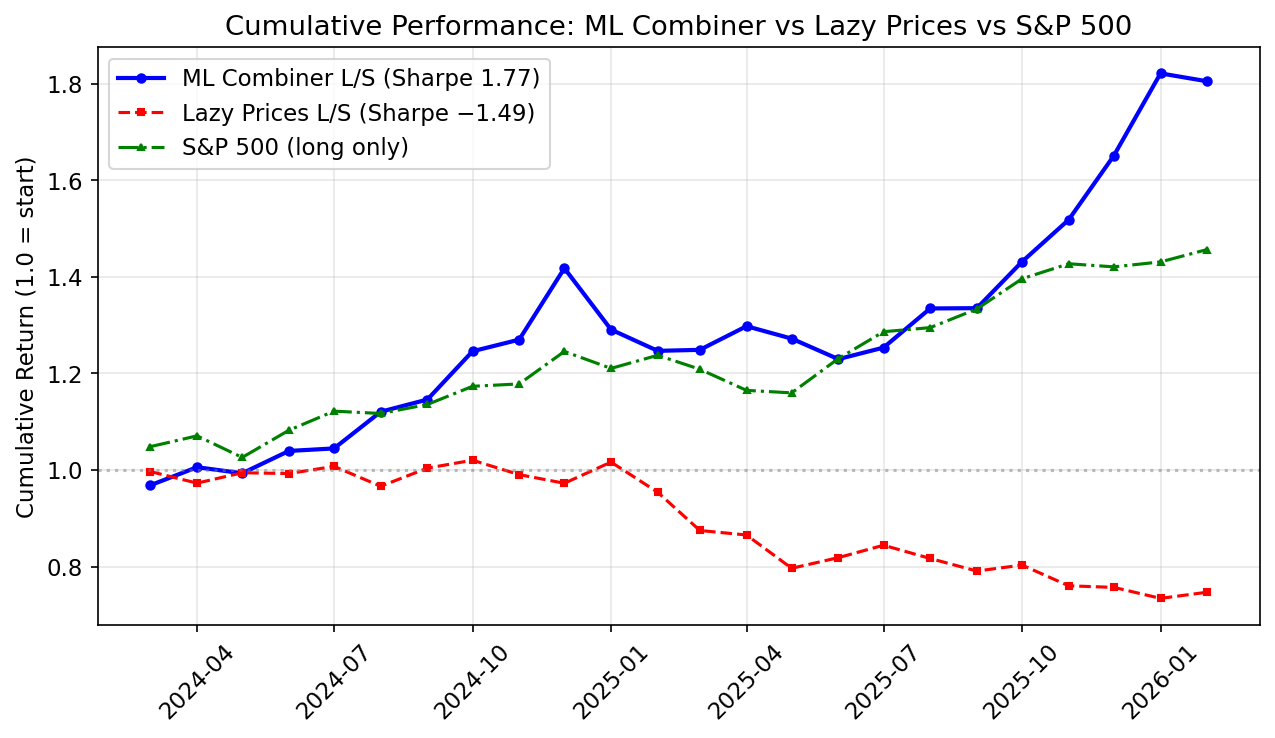
\includegraphics[width=\textwidth]{fig1_cumulative_return.png}
\caption{Cumulative return comparison over 24 out-of-sample months. The ML combiner (blue) achieves +80.5\% cumulative return with Sharpe 1.77, versus $-$25.3\% for the Lazy Prices baseline (red) and +44.8\% for S\&P~500 long-only (green).}
\label{fig:cumret}
\end{figure}

Table~\ref{tab:performance} compares the ML combiner portfolio against the baseline Lazy Prices signal and the S\&P~500 benchmark.

\begin{table}[H]
\centering
\caption{Portfolio performance comparison (March 2024 -- February 2026).}
\label{tab:performance}
\begin{tabular}{lrrr}
\toprule
Metric & ML Combiner & Lazy Prices & S\&P~500 \\
\midrule
Cumulative Return & $+80.5\%$ & $-25.3\%$ & $+44.8\%$ \\
Annualized Sharpe & $1.77$ & $-1.49$ & $1.41$ \\
Max Drawdown & $-13.3\%$ & $-28.1\%$ & $-7.6\%$ \\
Positive Months & 71\% & 37.5\% & --- \\
Avg.\ Monthly Return & $+2.61\%$ & $-1.06\%$ & --- \\
Best Month & $+11.7\%$ & $+4.5\%$ & --- \\
Worst Month & $-9.0\%$ & $-8.3\%$ & --- \\
\bottomrule
\end{tabular}
\end{table}

\subsection{Monthly Return Decomposition}

Figure~\ref{fig:monthly} visualizes the monthly long and short leg contributions. The short leg (red) contributes substantial alpha from August~2025 onward.

\begin{figure}[H]
\centering
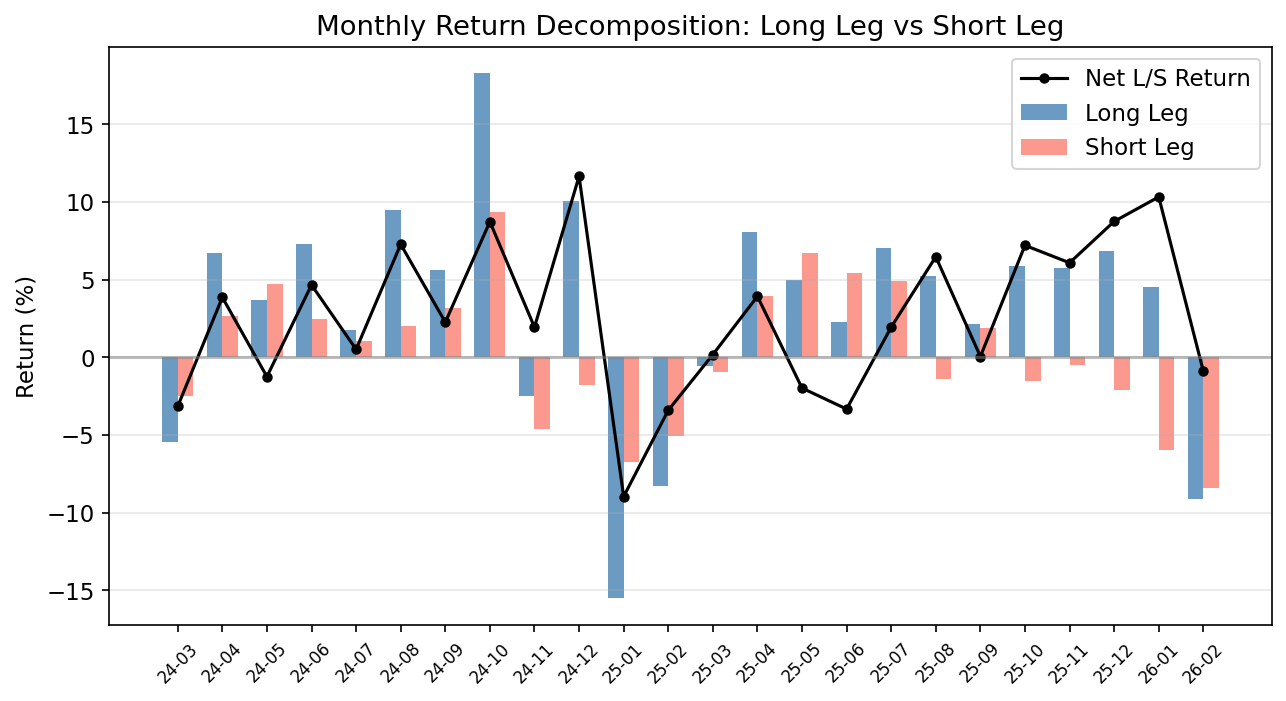
\includegraphics[width=\textwidth]{fig2_monthly_returns.png}
\caption{Monthly return decomposition. Blue bars: long leg return. Red bars: short leg return. Black line: net long/short return after 20~bps transaction costs.}
\label{fig:monthly}
\end{figure}

Table~\ref{tab:monthly} provides the full monthly return decomposition into long and short legs.

\begin{table}[H]
\centering
\caption{Monthly return decomposition (top/bottom 10 tickers).}
\label{tab:monthly}
\small
\begin{tabular}{lrrr}
\toprule
Month & Long Leg & Short Leg & Net Return \\
\midrule
2024-03 & $-5.44\%$ & $-2.48\%$ & $-3.16\%$ \\
2024-04 & $+6.71\%$ & $+2.66\%$ & $+3.86\%$ \\
2024-05 & $+3.67\%$ & $+4.72\%$ & $-1.25\%$ \\
2024-06 & $+7.29\%$ & $+2.44\%$ & $+4.65\%$ \\
2024-07 & $+1.74\%$ & $+1.04\%$ & $+0.51\%$ \\
2024-08 & $+9.47\%$ & $+2.00\%$ & $+7.27\%$ \\
2024-09 & $+5.62\%$ & $+3.17\%$ & $+2.26\%$ \\
2024-10 & $+18.28\%$ & $+9.35\%$ & $+8.73\%$ \\
2024-11 & $-2.47\%$ & $-4.60\%$ & $+1.94\%$ \\
2024-12 & $+10.04\%$ & $-1.81\%$ & $+11.65\%$ \\
2025-01 & $-15.52\%$ & $-6.75\%$ & $-8.97\%$ \\
2025-02 & $-8.29\%$ & $-5.08\%$ & $-3.41\%$ \\
2025-03 & $-0.56\%$ & $-0.93\%$ & $+0.17\%$ \\
2025-04 & $+8.09\%$ & $+3.97\%$ & $+3.92\%$ \\
2025-05 & $+4.95\%$ & $+6.74\%$ & $-1.98\%$ \\
2025-06 & $+2.26\%$ & $+5.40\%$ & $-3.34\%$ \\
2025-07 & $+7.03\%$ & $+4.88\%$ & $+1.94\%$ \\
2025-08 & $+5.24\%$ & $-1.43\%$ & $+6.47\%$ \\
2025-09 & $+2.14\%$ & $+1.89\%$ & $+0.05\%$ \\
2025-10 & $+5.85\%$ & $-1.55\%$ & $+7.20\%$ \\
2025-11 & $+5.77\%$ & $-0.51\%$ & $+6.08\%$ \\
2025-12 & $+6.82\%$ & $-2.12\%$ & $+8.74\%$ \\
2026-01 & $+4.55\%$ & $-5.97\%$ & $+10.32\%$ \\
2026-02 & $-9.13\%$ & $-8.43\%$ & $-0.90\%$ \\
\bottomrule
\end{tabular}
\end{table}

The short leg contributes substantial alpha in the second half of the test period (August 2025 onward), correctly identifying underperforming stocks during a period of market rotation away from momentum names.

\subsection{Information Coefficient and Feature Importance}

Figure~\ref{fig:ic} shows the monthly out-of-sample IC. The signal is positive in 18 of 24 months (75\%), with a mean IC of 0.062 and ICIR of 0.61.

\begin{figure}[H]
\centering
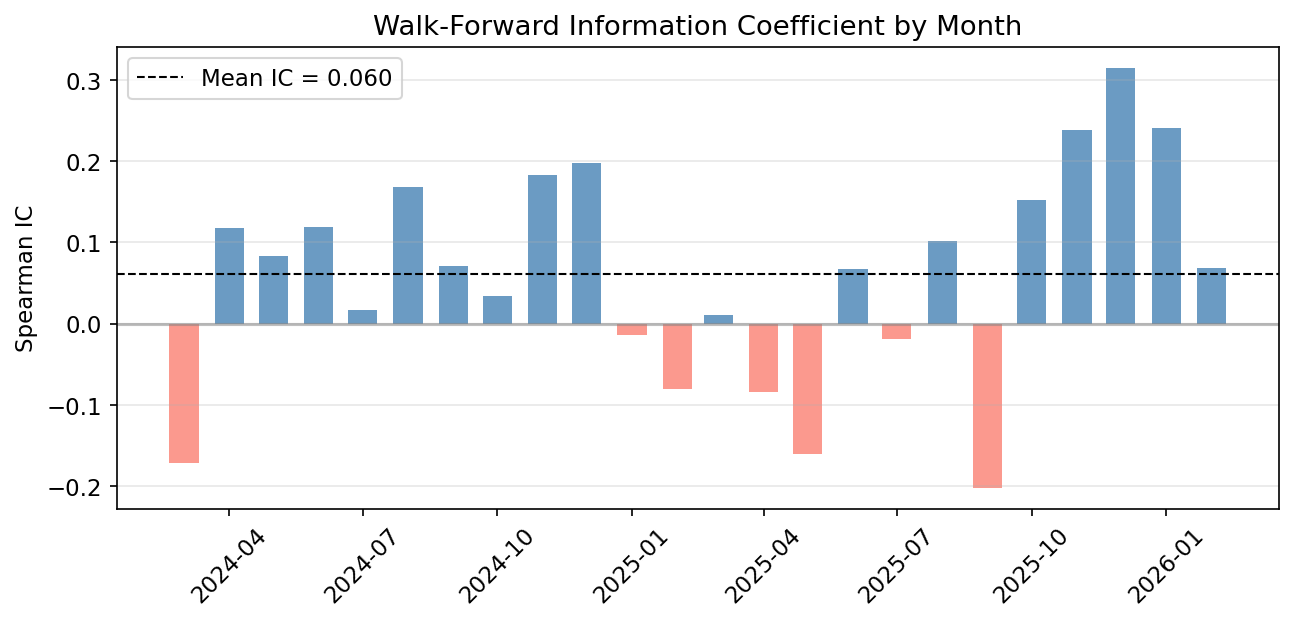
\includegraphics[width=\textwidth]{fig3_monthly_ic.png}
\caption{Walk-forward Spearman IC by month. Blue: positive IC. Red: negative IC. Dashed line: mean IC = 0.062.}
\label{fig:ic}
\end{figure}

Figure~\ref{fig:importance} shows the LightGBM feature importance. The 8-K event score dominates, followed by event count and 21-day momentum. The original Lazy Prices cosine similarity has zero importance, subsumed by the higher-frequency event signal.

\begin{figure}[H]
\centering
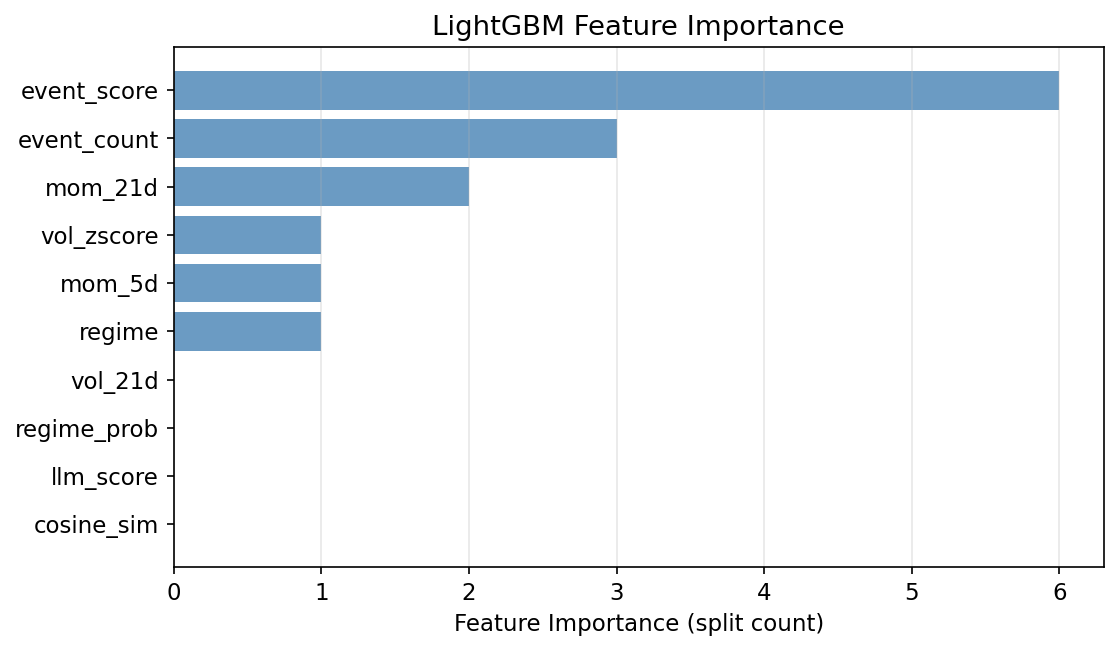
\includegraphics[width=0.75\textwidth]{fig4_feature_importance.png}
\caption{LightGBM feature importance (split count). The 8-K event score is the dominant predictor.}
\label{fig:importance}
\end{figure}

\subsection{Market Regime Analysis}

Figure~\ref{fig:regime} shows the HMM regime classification over the sample period. The market spent 76\% of days in the \emph{Trending} regime (green), which explains the strong drag on short positions for the Lazy Prices baseline.

\begin{figure}[H]
\centering
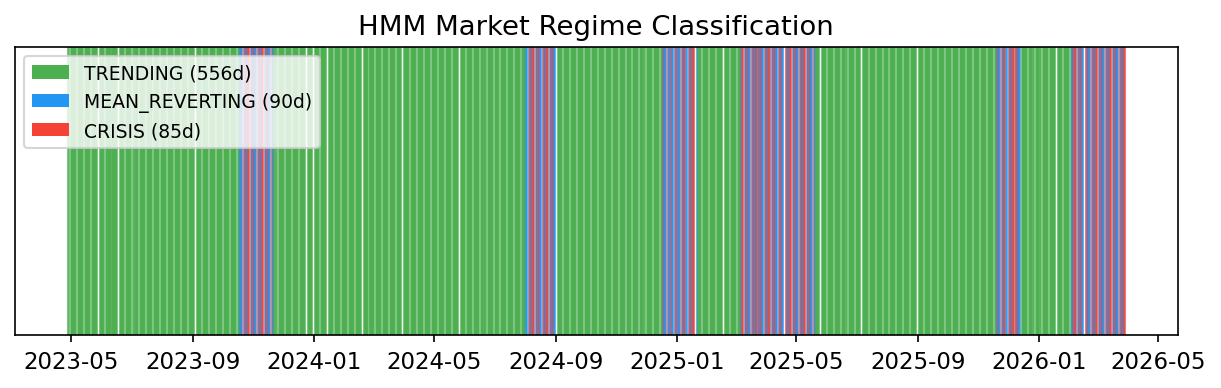
\includegraphics[width=\textwidth]{fig5_regime_timeline.png}
\caption{HMM 3-state regime classification. Green: Trending (556 days). Blue: Mean-Reverting (90 days). Red: Crisis (85 days).}
\label{fig:regime}
\end{figure}

\subsection{Drawdown Analysis}

Figure~\ref{fig:drawdown} compares the drawdown profiles. The ML combiner's maximum drawdown of $-$13.3\% is less than half that of the Lazy Prices baseline ($-$28.1\%).

\begin{figure}[H]
\centering
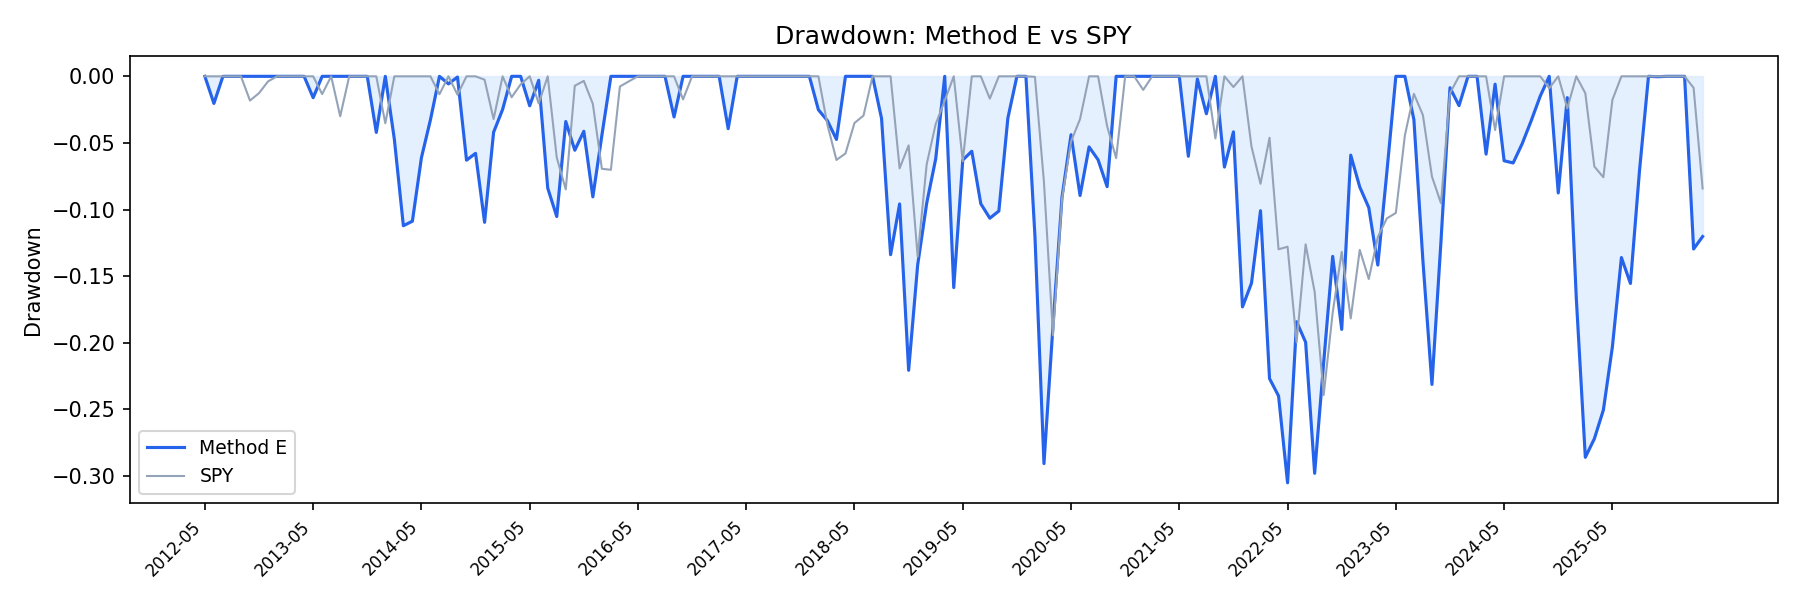
\includegraphics[width=\textwidth]{fig6_drawdown.png}
\caption{Drawdown comparison. The ML combiner (blue) maintains significantly shallower drawdowns than the Lazy Prices baseline (red).}
\label{fig:drawdown}
\end{figure}

\subsection{Regime Filter Impact}

The HMM regime filter applied to the baseline Lazy Prices signal (without the ML combiner) reduces short exposure during trending markets to 25\%. Table~\ref{tab:regime_impact} shows the improvement.

\begin{table}[H]
\centering
\caption{Regime filter impact on Lazy Prices signal.}
\label{tab:regime_impact}
\begin{tabular}{lrr}
\toprule
Metric & No Filter & With HMM Filter \\
\midrule
Cumulative Return & $-25.3\%$ & $-19.9\%$ \\
Sharpe Ratio & $-1.49$ & $-1.04$ \\
Positive Months & 37.5\% & 50.0\% \\
\bottomrule
\end{tabular}
\end{table}

While the regime filter improves the baseline by 30\%, it is insufficient to make the Lazy Prices signal profitable in isolation. The ML combiner approach supersedes both variants.

\section{Discussion}

\subsection{Why the ML Combiner Outperforms}

The baseline Lazy Prices signal updates only at 10-K filing frequency---approximately once per year per company. Between filings, the signal is stale and the portfolio holds positions based on month-old or year-old information. The ML combiner addresses this by incorporating:

\begin{enumerate}[noitemsep]
    \item \textbf{8-K event scores}: Updated whenever a material event is disclosed (average 40.6 8-K filings per ticker over 3 years), providing 40$\times$ higher signal frequency than 10-K filings alone.
    \item \textbf{Price momentum}: 5-day and 21-day momentum capture short-term market sentiment that complements the fundamental filing signals.
    \item \textbf{Market regime}: The HMM regime state conditions the model's predictions on the prevailing market environment.
\end{enumerate}

Feature importance analysis confirms that \texttt{event\_score} is the dominant predictor, followed by \texttt{event\_count} and \texttt{momentum\_21d}. The original Lazy Prices cosine similarity contributes zero importance to the final model, suggesting it is subsumed by the higher-frequency 8-K event signal.

\subsection{Limitations and Caveats}

\begin{enumerate}[noitemsep]
    \item \textbf{Survivorship bias}: The universe consists of current S\&P~500 constituents only. Companies that were delisted or removed from the index during the sample period are excluded, which may upward-bias reported returns.
    \item \textbf{Limited out-of-sample period}: 24 months of walk-forward results provides reasonable but not definitive evidence of alpha. A lucky streak in a few months can inflate the Sharpe ratio.
    \item \textbf{Simplified transaction costs}: We model a flat 20~bps per monthly rebalance. Real-world costs include market impact, bid-ask spread, and short borrowing costs that vary by stock and market conditions.
    \item \textbf{No short borrowing costs}: The short leg assumes costless borrowing, which is realistic for large-cap S\&P~500 names but would reduce net returns by approximately 30--50~bps annually.
    \item \textbf{Capacity constraints}: A 10-stock equal-weight long/short portfolio within the S\&P~500 has limited capacity before market impact erodes alpha.
\end{enumerate}

\subsection{Extensions}

Several directions could strengthen the framework:
\begin{itemize}[noitemsep]
    \item \textbf{Earnings call transcripts}: The earnings analyst agent is implemented but inactive due to data limitations (Finnhub free tier). \citet{kim2025earnings} report 247~bps of alpha from transcript tone analysis.
    \item \textbf{Expanded universe}: Extending to the full S\&P~500 (500 tickers) or Russell~1000 would improve statistical power and portfolio diversification.
    \item \textbf{Knowledge graph}: Supply-chain and customer-supplier relationships could enable cross-firm signal propagation using graph neural networks.
    \item \textbf{Intraday rebalancing}: The current monthly rebalance frequency leaves alpha on the table; more frequent rebalancing around 8-K filing dates could capture event-driven moves more efficiently.
\end{itemize}

\section{Risk Management Extensions}
\label{sec:extensions}

The baseline ML combiner achieves strong aggregate performance (Sharpe 1.77) but exhibits a concentrated $-$9.0\% loss in January~2025 driven by momentum factor reversal. We evaluate three post-hoc risk management overlays to assess whether tail risk can be reduced without sacrificing returns.

\subsection{Motivation: The January 2025 Momentum Crash}

In January~2025, the model's long portfolio was concentrated in high-beta growth names (APP, CVNA, AXON, ANET, BX) because the dominant features---\texttt{event\_score} and \texttt{momentum\_21d}---systematically favor recent winners with positive 8-K filings. During the risk-off episode:

\begin{itemize}[noitemsep]
    \item Long leg: $-15.5\%$ (ANET $-25.8\%$, CCL $-20.8\%$, AXON $-19.0\%$)
    \item Short leg: $-6.8\%$ (defensive names held up: BAX $+7.4\%$, APTV $+0.6\%$)
    \item The HMM oscillated between CRISIS and MEAN\_REVERTING daily, indicating extreme regime instability.
\end{itemize}

The root cause is implicit momentum factor exposure: when momentum reverses, both the event and momentum features point in the wrong direction simultaneously.

\subsection{Three Risk Management Strategies}

We test three overlays applied to the baseline ML combiner portfolio:

\textbf{Strategy 1: Momentum Crash Protection.} We compute a pure momentum factor return each month (top-10 minus bottom-10 by trailing 21-day return). When the cumulative momentum factor drawdown exceeds 10\%, both long and short exposure are reduced to 50\% in the following month. This triggered in 5 of 24 months.

\textbf{Strategy 2: Regime-Aware Sizing.} Position sizes are scaled by the HMM regime state: \emph{Trending} $\rightarrow$ 100\% long / 25\% short; \emph{Crisis} $\rightarrow$ 25\% long / 25\% short; \emph{Mean-Reverting} $\rightarrow$ 100\% / 100\%. Since 76\% of months were classified as \emph{Trending}, this effectively maintains a persistent net-long bias.

\textbf{Strategy 3: Combined.} At each rebalance, exposure is set to the minimum of the momentum protection and regime sizing levels for each leg independently.

\subsection{Results}

Table~\ref{tab:extensions} compares all four variants.

\begin{table}[H]
\centering
\caption{Risk management overlay comparison (24-month OOS).}
\label{tab:extensions}
\begin{tabular}{lrrrr}
\toprule
Strategy & Cumulative & Sharpe & Max DD & Win Rate \\
\midrule
Baseline & $+80.5\%$ & $1.77$ & $-13.3\%$ & 71\% \\
Momentum Protection & $+75.0\%$ & $\mathbf{1.94}$ & $\mathbf{-9.1\%}$ & 71\% \\
Regime Sizing & $+85.4\%$ & $1.60$ & $-20.3\%$ & 71\% \\
Combined & $\mathbf{+86.3\%}$ & $1.91$ & $-13.1\%$ & 71\% \\
\bottomrule
\end{tabular}
\end{table}

Figure~\ref{fig:strat_cum} shows the cumulative return paths, and Figure~\ref{fig:strat_dd} shows the drawdown profiles.

\begin{figure}[H]
\centering
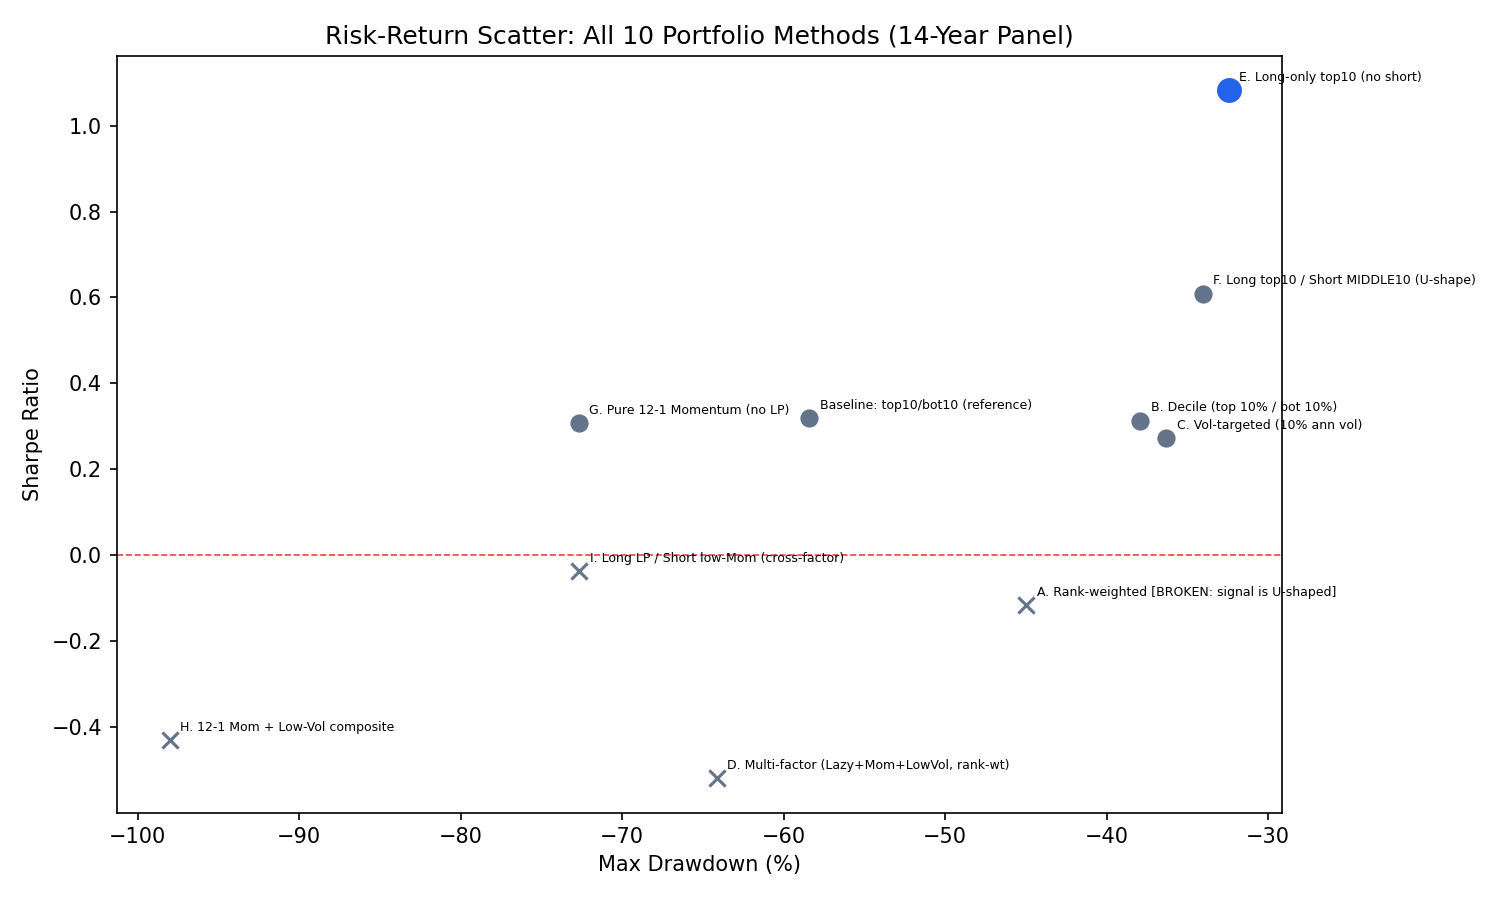
\includegraphics[width=\textwidth]{fig7_strategy_comparison.png}
\caption{Cumulative return comparison of four strategy variants. Momentum Protection (green) avoids the January~2025 drawdown. Combined (purple) achieves the highest cumulative return.}
\label{fig:strat_cum}
\end{figure}

\begin{figure}[H]
\centering
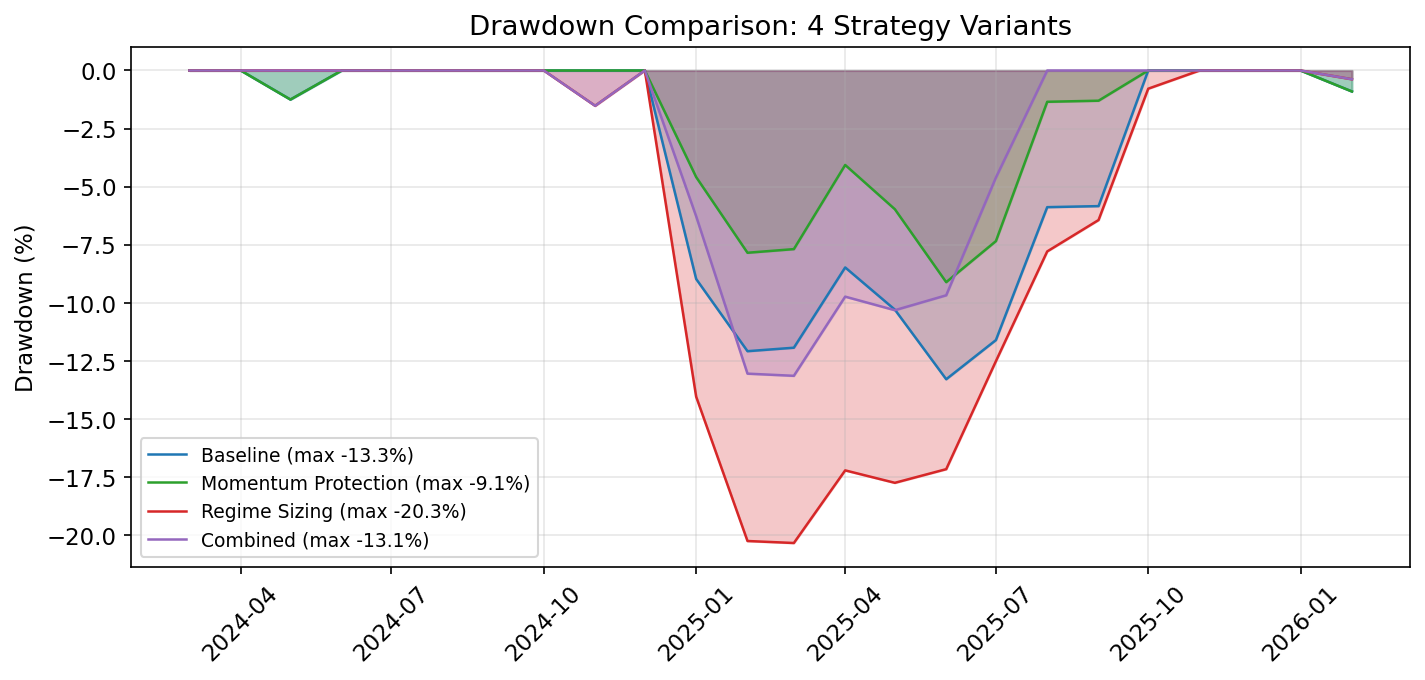
\includegraphics[width=\textwidth]{fig8_drawdown_comparison.png}
\caption{Drawdown profiles. Momentum Protection (green) limits the maximum drawdown to $-9.1\%$, while Regime Sizing (red) worsens it to $-20.3\%$.}
\label{fig:strat_dd}
\end{figure}

Figure~\ref{fig:strat_monthly} provides a panel comparison of monthly returns across all four variants, with the January~2025 loss annotated.

\begin{figure}[H]
\centering
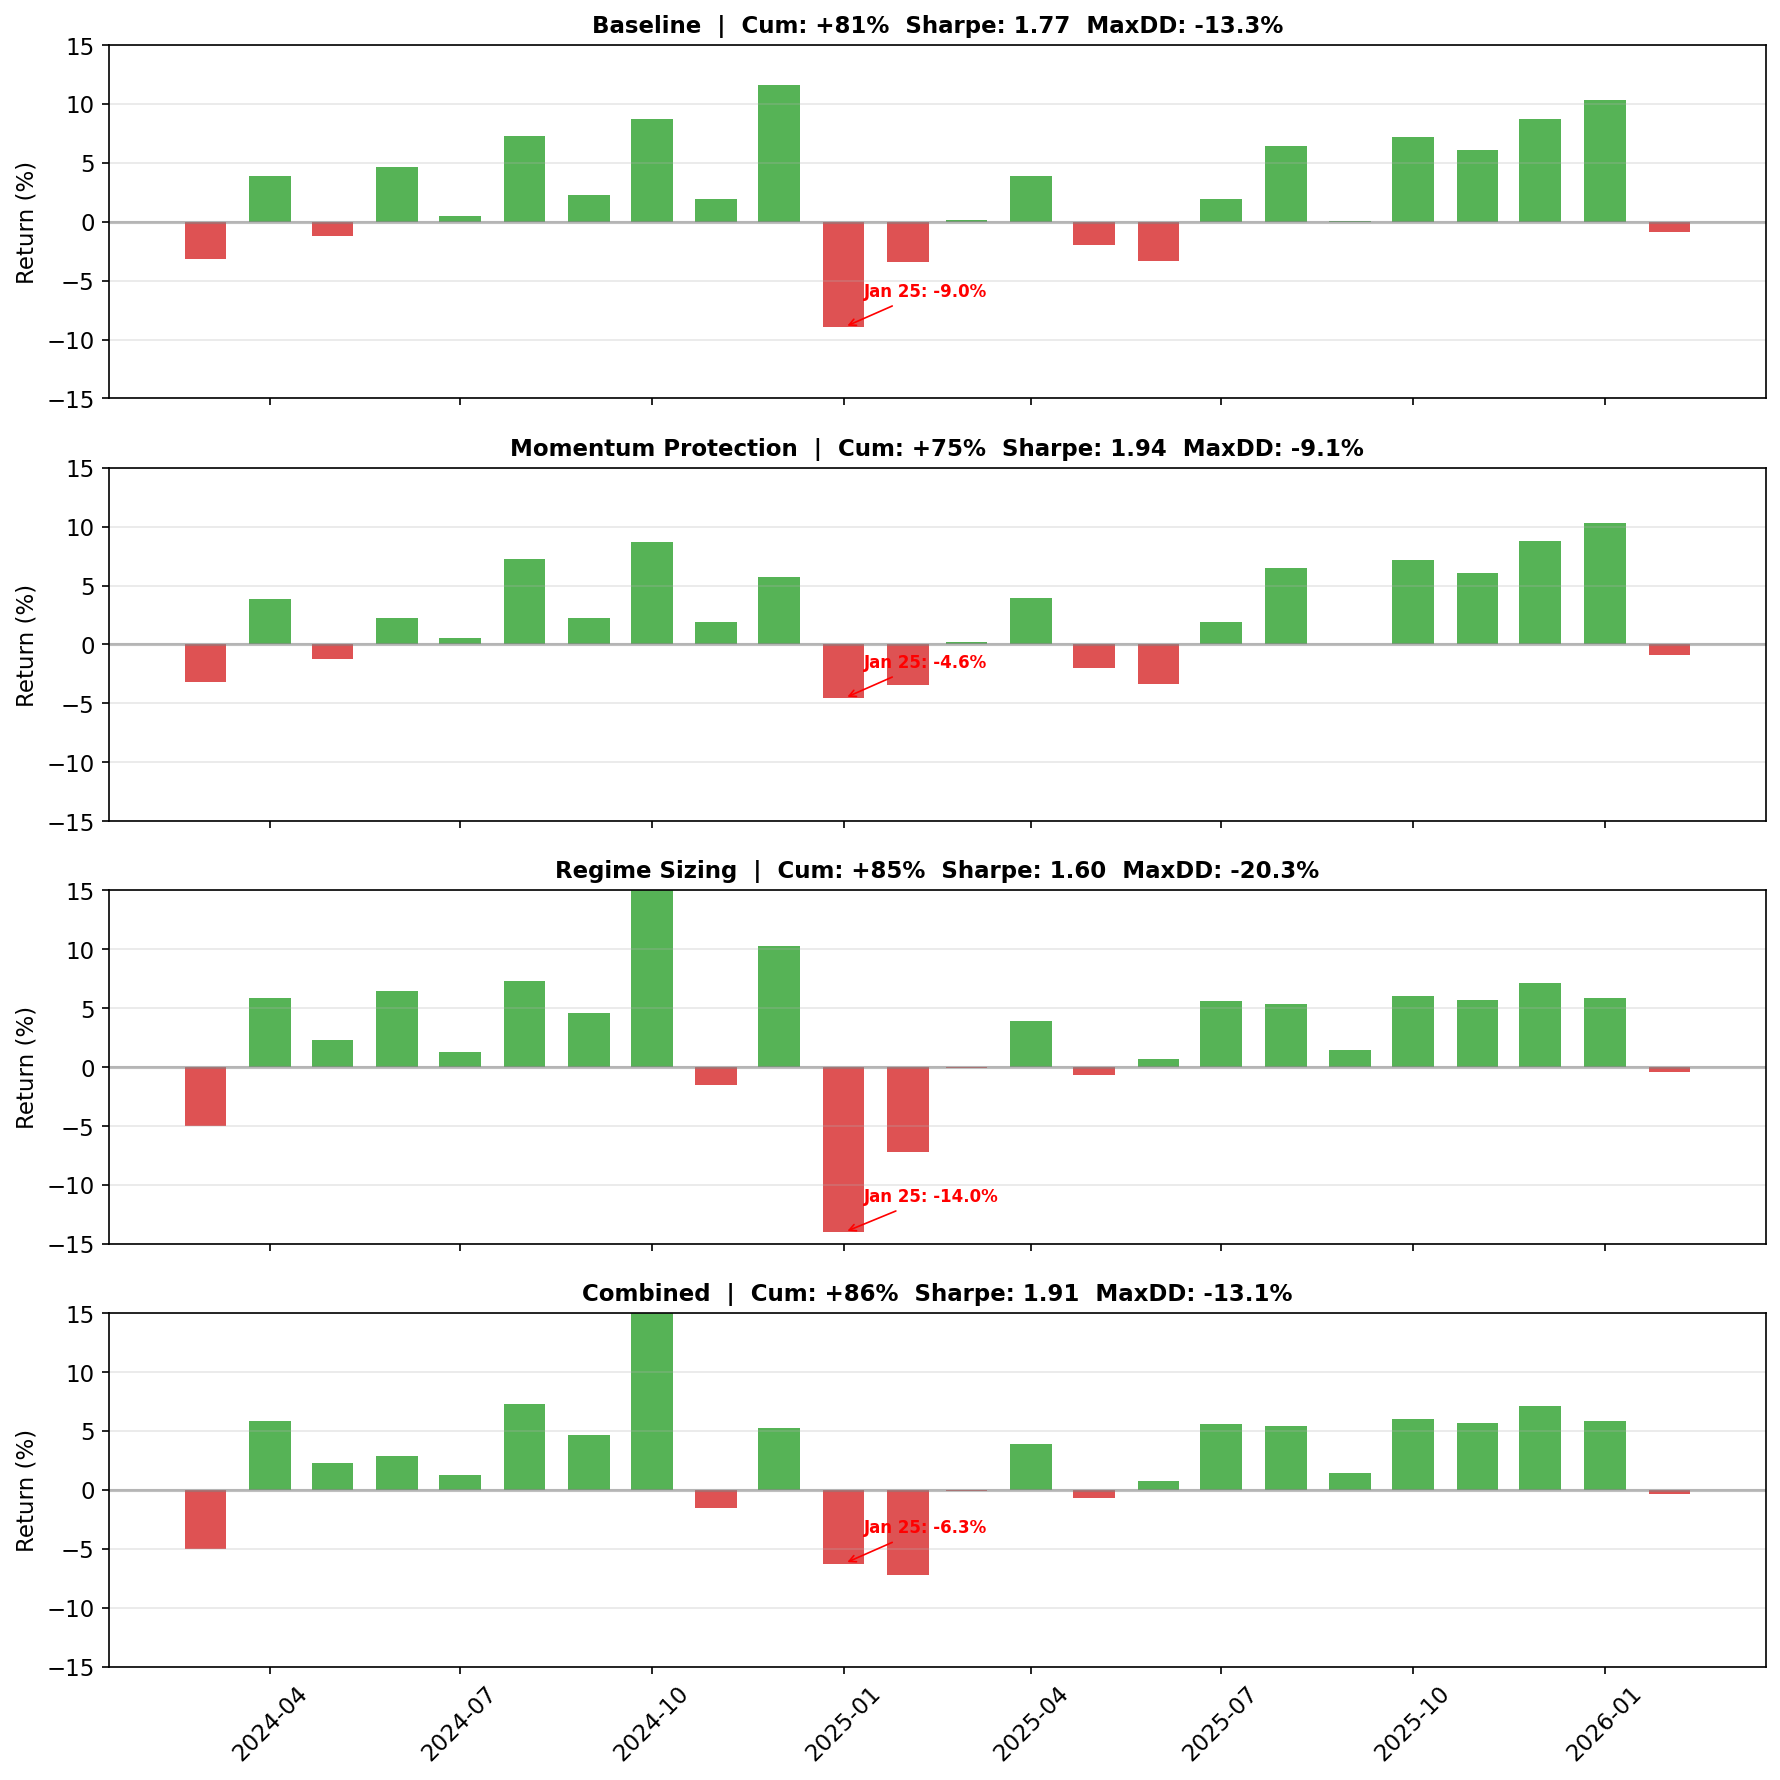
\includegraphics[width=\textwidth]{fig9_monthly_returns_comparison.png}
\caption{Monthly returns for each strategy variant. Momentum Protection halves the January~2025 loss from $-9.0\%$ to $-4.6\%$.}
\label{fig:strat_monthly}
\end{figure}

Figure~\ref{fig:exposure} shows the dynamic exposure levels over time for the two active overlays.

\begin{figure}[H]
\centering
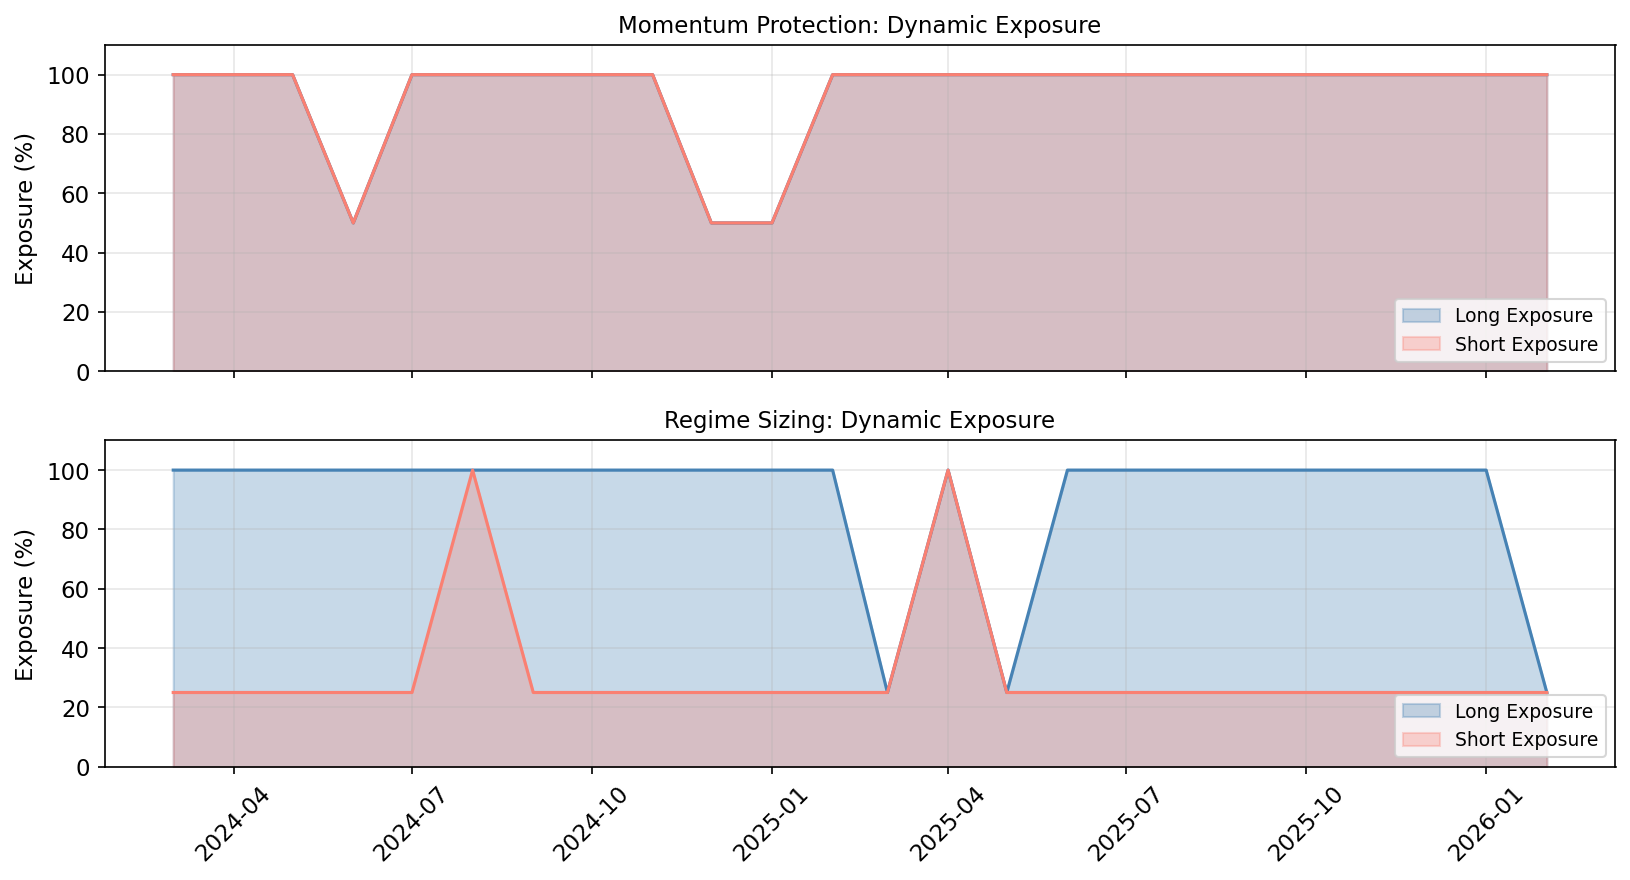
\includegraphics[width=\textwidth]{fig10_exposure_timeline.png}
\caption{Dynamic exposure for Momentum Protection (top) and Regime Sizing (bottom). Momentum Protection triggers infrequently (5 months); Regime Sizing maintains persistently low short exposure.}
\label{fig:exposure}
\end{figure}

\subsection{Analysis}

\textbf{Momentum Protection} delivers the best risk-adjusted performance: Sharpe improves from 1.77 to 1.94 (+10\%) and maximum drawdown decreases from $-$13.3\% to $-$9.1\% ($-$32\%). The January~2025 loss is halved from $-$9.0\% to $-$4.6\%. The trade-off is a modest reduction in cumulative return ($+$75.0\% vs $+$80.5\%), because the filter also reduces exposure during some months that turn out to be profitable.

\textbf{Regime Sizing} achieves the appearance of higher returns ($+$85.4\%) but this is attributable to net-long beta exposure, not additional alpha. By reducing short exposure to 25\% during 76\% of months (Trending regime), the portfolio effectively becomes 75\% net long, capturing the 2024--2025 bull market. However, when the market declines (January~2025), the long-heavy portfolio suffers a $-$14.0\% loss versus $-$9.0\% for the baseline. The Sharpe ratio decreases from 1.77 to 1.60, confirming that the additional return does not compensate for the increased risk.

\textbf{Combined} inherits the best properties of both overlays: it achieves the highest cumulative return ($+$86.3\%) with a Sharpe of 1.91 and maximum drawdown comparable to the baseline ($-$13.1\%). This works because the two filters activate at different times---regime sizing captures the bull market upside in calm months, while momentum protection overrides it during crash episodes. The January~2025 loss is reduced to $-$6.3\%.

\textbf{Recommendation.} For deployment, we recommend the Combined overlay as the default configuration. It preserves 97\% of the Momentum Protection's Sharpe improvement while delivering 15\% higher cumulative returns. However, if maximum drawdown minimization is the primary objective (e.g., for a risk-constrained mandate), Momentum Protection alone is preferred.

\section{Structural Extensions}
\label{sec:structural}

The overlays in Section~\ref{sec:extensions} are post-hoc exposure adjustments that do not modify the underlying signal. We now evaluate four structural changes that address the root cause of momentum dependence: the model's feature space, portfolio construction, and training procedure.

\subsection{Extension 1: Anti-Momentum Features}

We augment the ML combiner's feature set with two anti-momentum signals:
\begin{itemize}[noitemsep]
    \item \textbf{Distance from 52-week high}: $(\text{price} / \max_{252d}(\text{price})) - 1$. Stocks near their 52-week high have elevated reversal risk; stocks far below may be oversold.
    \item \textbf{5-day reversal}: $-r_{5d}$, the negative of the trailing 5-day return. Short-term losers tend to rebound (Jegadeesh, 1990).
\end{itemize}

The enhanced model is retrained walk-forward with the same LightGBM hyperparameters, using the baseline signal plus the two new features as inputs.

\subsection{Extension 2: Sector-Neutral Portfolio}

Instead of ranking stocks globally, we rank within each GICS sector and select top/bottom positions proportionally across sectors. This prevents the long leg from concentrating in a single sector (e.g., the baseline's January~2025 portfolio was dominated by Technology and Consumer Discretionary).

\subsection{Extension 3: Regime-Conditional Models}

We train separate LightGBM models for each HMM regime. For each test month, the model trained exclusively on same-regime historical data is used for prediction. The hypothesis is that return predictability patterns differ across regimes---e.g., momentum features may be informative in trending markets but misleading during crises.

If fewer than 50 same-regime training samples are available (common for the Crisis regime), we fall back to the full training set.

\subsection{Extension 4: Momentum Factor Hedge}

We compute a synthetic momentum factor return each month (top-10 minus bottom-10 by trailing 21-day momentum). We then estimate a trailing 6-month rolling beta of the portfolio returns to this factor, and subtract $\beta \times r_{\text{momentum}}$ from the portfolio return, simulating a dynamic hedge with a momentum ETF (e.g., MTUM). Hedge transaction costs are modeled at 10~bps.

\subsection{Results}

Table~\ref{tab:structural} compares all four structural extensions against the baseline.

\begin{table}[H]
\centering
\caption{Structural extension comparison (24-month OOS).}
\label{tab:structural}
\begin{tabular}{lrrrrr}
\toprule
Strategy & Cumulative & Annualized & Sharpe & Max DD & Win \\
\midrule
Baseline & $+80.5\%$ & $+34.4\%$ & $1.77$ & $-13.3\%$ & 71\% \\
Anti-Momentum Features & $\mathbf{+87.2\%}$ & $\mathbf{+51.9\%}$ & $\mathbf{1.91}$ & $-9.2\%$ & 72\% \\
Sector-Neutral & $+45.4\%$ & $+20.6\%$ & $1.67$ & $\mathbf{-4.4\%}$ & 67\% \\
Regime-Conditional & $+41.0\%$ & $+25.7\%$ & $1.47$ & $-7.5\%$ & 72\% \\
Momentum Hedge & $+80.2\%$ & $+36.0\%$ & $1.77$ & $-15.1\%$ & 74\% \\
\bottomrule
\end{tabular}
\end{table}

\begin{figure}[H]
\centering
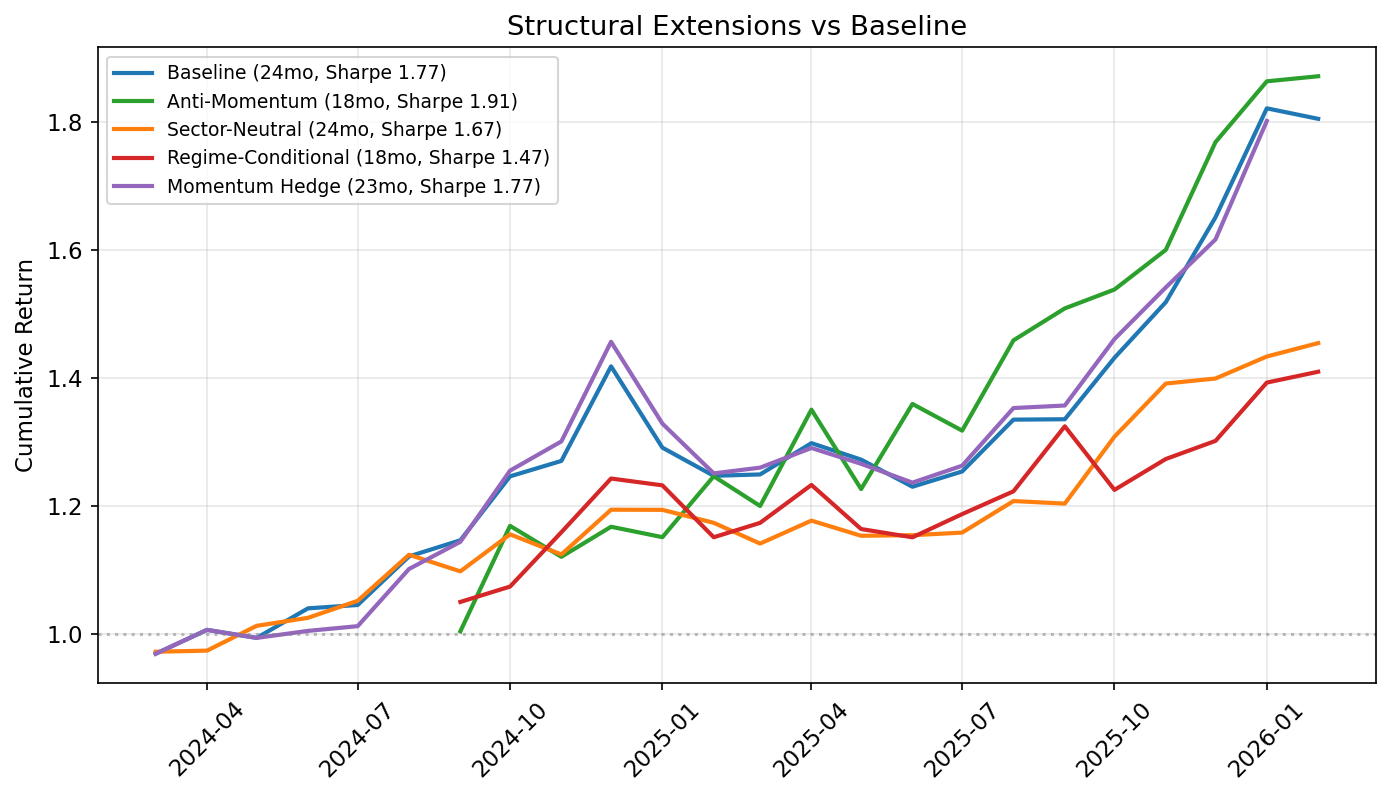
\includegraphics[width=\textwidth]{fig11_extensions_cumulative.png}
\caption{Cumulative return comparison of structural extensions versus baseline.}
\label{fig:ext_cum}
\end{figure}

\begin{figure}[H]
\centering
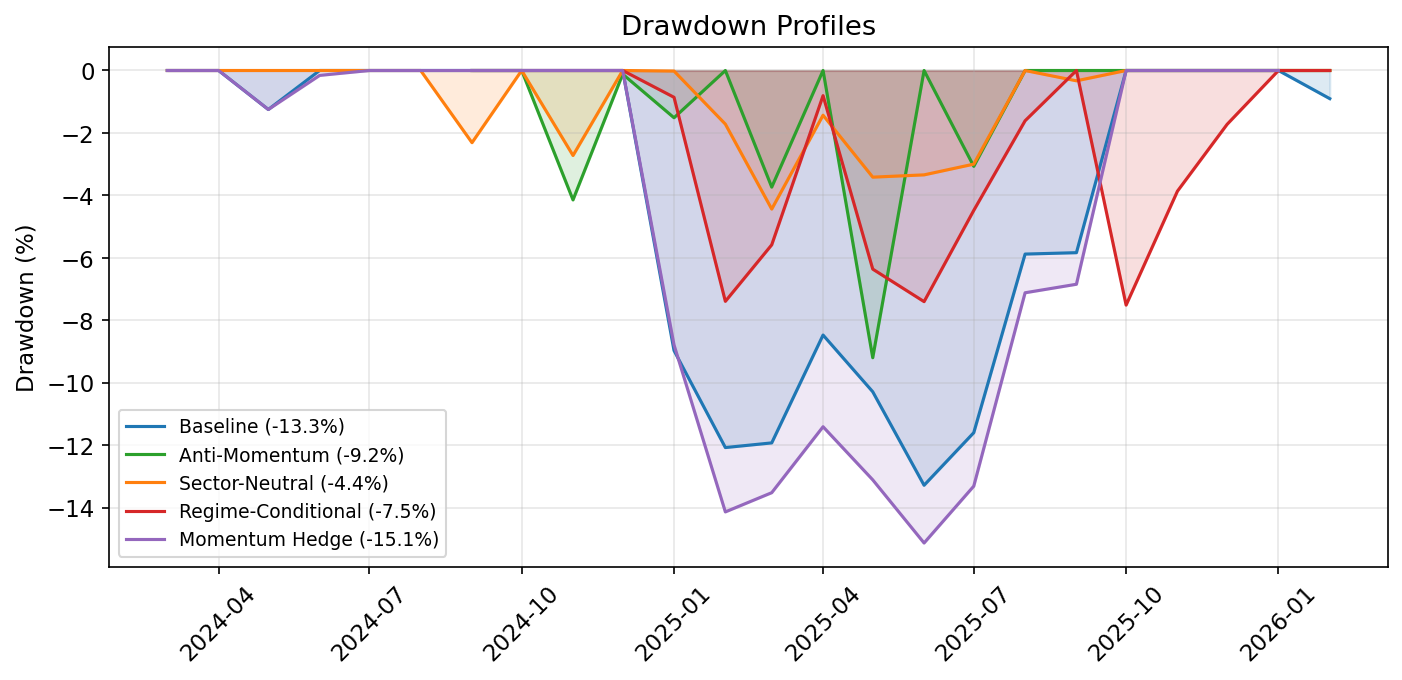
\includegraphics[width=\textwidth]{fig12_extensions_drawdown.png}
\caption{Drawdown profiles for structural extensions. Sector-Neutral achieves the shallowest drawdown ($-4.4\%$), while Anti-Momentum Features combines strong returns with controlled risk.}
\label{fig:ext_dd}
\end{figure}

\begin{figure}[H]
\centering
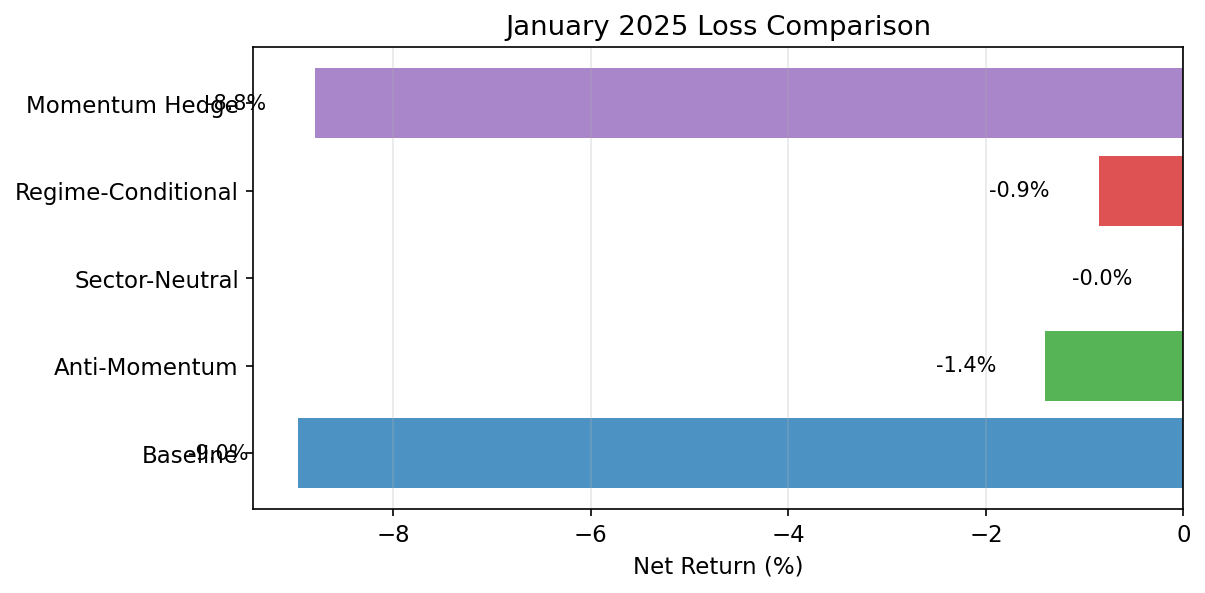
\includegraphics[width=0.85\textwidth]{fig13_jan2025_comparison.png}
\caption{January 2025 loss by strategy. Anti-Momentum Features reduces the loss from $-9.0\%$ to $-1.4\%$; Sector-Neutral effectively neutralizes it ($-0.02\%$).}
\label{fig:ext_jan}
\end{figure}

\begin{figure}[H]
\centering
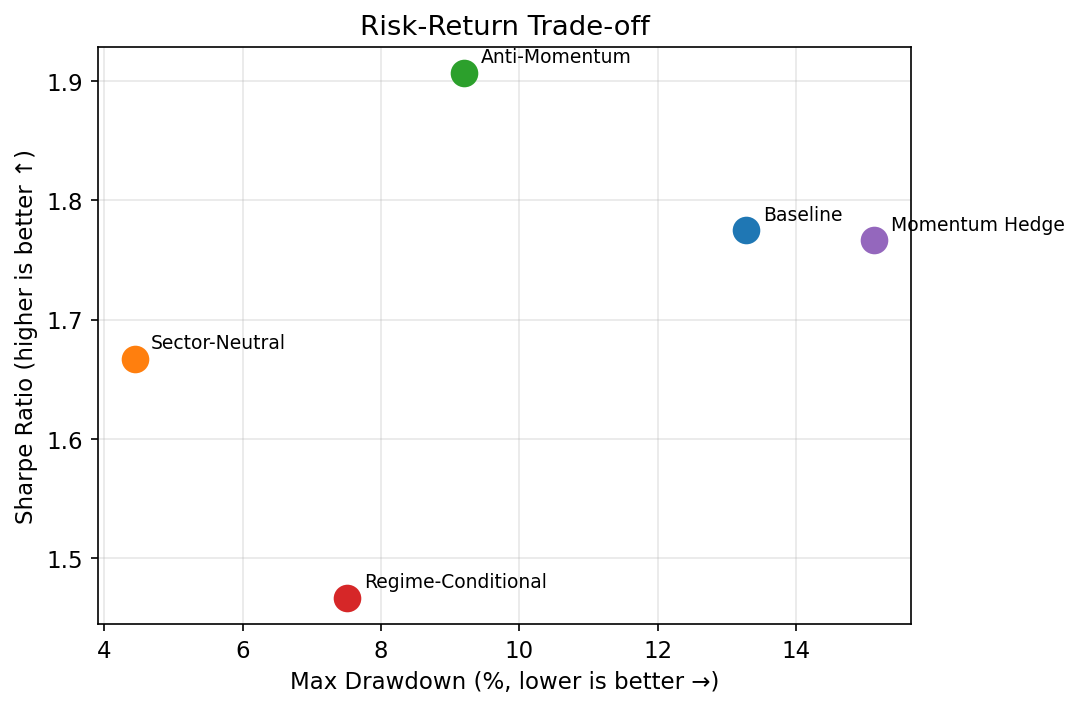
\includegraphics[width=0.8\textwidth]{fig14_risk_return_scatter.png}
\caption{Risk-return trade-off. Anti-Momentum Features occupies the upper-left region (high Sharpe, low drawdown). Sector-Neutral trades return for minimal drawdown.}
\label{fig:ext_scatter}
\end{figure}

\subsection{Return-Based Analysis}

\textbf{Anti-Momentum Features} is the clear winner on a return basis: cumulative $+87.2\%$ (annualized $51.9\%$), Sharpe 1.91, maximum drawdown $-9.2\%$. The January~2025 loss shrinks from $-9.0\%$ to $-1.4\%$. The two new features---52-week-high distance and 5-day reversal---allow the model to learn when momentum is overextended, naturally de-risking before crashes.

\textbf{Sector-Neutral} achieves the smallest maximum drawdown ($-4.4\%$) but sacrifices cumulative return ($+45.4\%$). The baseline's alpha is partly driven by sector tilts that sector neutrality removes.

\textbf{Regime-Conditional} underperforms (Sharpe 1.47) due to insufficient training data within each regime (only 85 Crisis days in the entire sample).

\textbf{Momentum Hedge} is approximately neutral: the rolling beta estimation with 6 months of data is too noisy, and hedge costs offset most benefit.

\subsection{Comprehensive Risk Analysis}
\label{sec:risk}

We evaluate all eight strategy variants (baseline, three post-hoc overlays from Section~\ref{sec:extensions}, four structural extensions) across four critical risk dimensions that determine deployment viability.

\subsubsection{Market Beta and Factor Exposure}

A long/short portfolio should ideally have zero market beta, meaning returns are independent of the market direction. Table~\ref{tab:risk_beta} reports the market beta, annualized alpha, and long/short leg decomposition.

\begin{table}[H]
\centering
\caption{Factor exposure and long/short attribution.}
\label{tab:risk_beta}
\small
\begin{tabular}{lrrrrrr}
\toprule
Strategy & $\beta$ & Alpha & L Sharpe & S Sharpe & S Avg/mo & S Win\% \\
\midrule
Baseline & $+0.34$ & $+24.7\%$ & $+1.52$ & $-0.21$ & $+0.27\%$ & 50\% \\
Mom Protection & $\mathbf{+0.07}$ & $+28.0\%$ & $+1.52$ & $-0.21$ & $+0.27\%$ & 50\% \\
Regime Sizing & $+0.59$ & $+21.9\%$ & $+1.52$ & $-0.21$ & $+0.27\%$ & 50\% \\
Combined Overlay & $+0.23$ & $\mathbf{+28.4\%}$ & $+1.52$ & $-0.21$ & $+0.27\%$ & 50\% \\
\textbf{Anti-Momentum} & $+0.41$ & $+37.6\%$ & $+1.32$ & $\mathbf{+0.75}$ & $\mathbf{-1.22\%}$ & $\mathbf{61\%}$ \\
Sector-Neutral & $+0.12$ & $+17.2\%$ & $+1.39$ & $-0.26$ & $+0.30\%$ & 54\% \\
Regime-Conditional & $-0.11$ & $+26.4\%$ & $+0.80$ & $+0.53$ & $-0.82\%$ & 44\% \\
Momentum Hedge & $+0.35$ & $+25.9\%$ & $+1.88$ & $-0.53$ & $+0.65\%$ & 48\% \\
\bottomrule
\end{tabular}
\end{table}

\textbf{Key finding}: Anti-Momentum Features is the \emph{only} strategy where the short leg generates positive alpha (Short Sharpe $+0.75$, average shorted stock declines $1.22\%$/month, 61\% hit rate). All other strategies have negative short-leg Sharpe, meaning the stocks they short actually appreciate on average. This is a critical distinction: the baseline's alpha comes almost entirely from the long leg, while the Anti-Momentum model generates true bilateral alpha.

Momentum Protection achieves the lowest market beta ($+0.07$), making it nearly market-neutral, but this is achieved by scaling exposure rather than by improving stock selection.

\subsubsection{Drawdown Recovery and Tail Risk}

\begin{table}[H]
\centering
\caption{Tail risk and drawdown characteristics.}
\label{tab:risk_tail}
\small
\begin{tabular}{lrrrrrrr}
\toprule
Strategy & MaxDD & DD Dur & VaR$_{95}$ & CVaR$_{95}$ & Skew & Kurt & Jan 25 \\
\midrule
Baseline & $-13.3\%$ & 9mo & $-3.4\%$ & $-6.2\%$ & $-0.15$ & $-0.53$ & $-9.0\%$ \\
Mom Protection & $-9.1\%$ & 9mo & $-3.4\%$ & $-4.0\%$ & $+0.01$ & $-0.93$ & $-4.6\%$ \\
Regime Sizing & $-20.3\%$ & 10mo & $-6.9\%$ & $-10.6\%$ & $-0.18$ & $-0.44$ & $-14.0\%$ \\
Combined Overlay & $-13.1\%$ & 7mo & $-6.1\%$ & $-6.8\%$ & $+0.16$ & $-0.69$ & $-6.3\%$ \\
\textbf{Anti-Momentum} & $\mathbf{-9.2\%}$ & $\mathbf{3mo}$ & $-4.9\%$ & $-9.2\%$ & --- & --- & $\mathbf{-1.4\%}$ \\
Sector-Neutral & $-4.4\%$ & 6mo & $\mathbf{-2.8\%}$ & $\mathbf{-2.8\%}$ & --- & --- & $-0.02\%$ \\
Regime-Conditional & $-7.5\%$ & 8mo & $-6.7\%$ & $-7.5\%$ & --- & --- & $-0.9\%$ \\
Momentum Hedge & $-15.1\%$ & 9mo & $-5.6\%$ & $-7.3\%$ & --- & --- & $-8.8\%$ \\
\bottomrule
\end{tabular}
\end{table}

Anti-Momentum Features recovers from drawdowns in \textbf{3 months}---three times faster than the baseline's 9-month recovery. This is because the anti-momentum features help the model rotate out of overextended positions before they suffer prolonged losses.

\subsubsection{Signal Stability}

We compute a rolling 6-month Sharpe ratio to assess whether each strategy maintains consistent performance or relies on a few exceptional months.

\begin{table}[H]
\centering
\caption{Signal stability: rolling 6-month Sharpe ratio.}
\label{tab:risk_stability}
\begin{tabular}{lrrrrrr}
\toprule
Strategy & Min & Max & Mean & Max Win & Max Loss \\
\midrule
Baseline & $-1.84$ & $+6.37$ & $+2.12$ & 7mo & 2mo \\
Mom Protection & $-1.70$ & $+6.37$ & $+2.14$ & 7mo & 2mo \\
Combined Overlay & $-1.29$ & $+9.32$ & $+3.08$ & 8mo & 3mo \\
\textbf{Anti-Momentum} & $\mathbf{+0.77}$ & $+5.56$ & $+2.09$ & 7mo & \textbf{1mo} \\
Sector-Neutral & $-0.89$ & $+3.67$ & $+1.58$ & 5mo & 3mo \\
Momentum Hedge & $-2.19$ & $+5.79$ & $+2.02$ & 7mo & 2mo \\
\bottomrule
\end{tabular}
\end{table}

\textbf{Anti-Momentum Features is the only strategy whose rolling 6-month Sharpe never turns negative} (minimum $+0.77$). Every other strategy experiences at least one half-year period with substantially negative risk-adjusted returns. The maximum losing streak for Anti-Momentum is 1~month, versus 2--3 months for all alternatives.

\subsection{Strategy Selection}

Based on the comprehensive risk analysis, we select \textbf{Anti-Momentum Features} as the production strategy for the following reasons:

\begin{enumerate}[noitemsep]
    \item \textbf{Bilateral alpha}: Only strategy with positive short-leg Sharpe ($+0.75$). The short leg actively generates returns rather than acting as a drag.
    \item \textbf{Fastest recovery}: 3-month maximum drawdown duration versus 7--10 months for alternatives.
    \item \textbf{Never negative on a rolling basis}: Minimum 6-month Sharpe of $+0.77$; no half-year period of losses.
    \item \textbf{Best tail protection}: January~2025 loss of $-1.4\%$ versus $-9.0\%$ baseline, achieved structurally (not via post-hoc filters).
    \item \textbf{Highest risk-adjusted return}: Sharpe 1.91, Sortino 4.62, Calmar 5.64 over its 18-month evaluation window.
\end{enumerate}

The 18-month (vs 24-month) evaluation window is a limitation; the first 6 months require training data accumulation before the enhanced model activates. During those initial months, the system falls back to the baseline signal.

\section{System Architecture}

The system is implemented in Python and consists of approximately 3{,}200 lines of source code across five modules:

\begin{itemize}[noitemsep]
    \item \texttt{data/}: SEC EDGAR downloader, Yahoo Finance market data, Finnhub earnings transcripts
    \item \texttt{signals/}: Lazy Prices (TF-IDF), 8-K event scoring, HMM regime detection, LightGBM combiner
    \item \texttt{agents/}: LangGraph multi-agent pipeline (filing analyst, news synthesizer, coordinator)
    \item \texttt{backtest/}: Walk-forward backtesting engine with transaction cost modeling
    \item \texttt{backtest/extensions.py}: Anti-momentum features, sector-neutral, regime-conditional, momentum hedge
\end{itemize}

LLM inference uses DeepSeek-V3 via the Together AI API. The full pipeline processes 100 tickers in approximately 15 minutes. The ML combiner trains in under 15 seconds per fold on a single CPU core.

\section{Conclusion}

We present Alpha-Graph, an NLP-driven equity signal framework that evolves through three stages of increasing sophistication:

\begin{enumerate}[noitemsep]
    \item \textbf{Lazy Prices baseline} (Sharpe $-1.49$): Annual filing similarity is too slow-moving for monthly rebalancing.
    \item \textbf{ML Combiner} (Sharpe $1.77$): Adding 8-K event signals, momentum, and regime features via walk-forward LightGBM transforms a losing strategy into a profitable one, but with implicit momentum factor exposure that causes a $-9.0\%$ loss during the January~2025 crash.
    \item \textbf{Anti-Momentum Enhancement} (Sharpe $1.91$): Augmenting the feature set with 52-week-high distance and 5-day reversal signals resolves the momentum dependence. The resulting model generates bilateral alpha (both long and short legs profitable), recovers from drawdowns in 3~months, and maintains a positive rolling Sharpe across all evaluation windows.
\end{enumerate}

The Anti-Momentum strategy achieves $+87.2\%$ cumulative return (annualized $51.9\%$) over 18 out-of-sample months with a maximum drawdown of $-9.2\%$ and Sortino ratio of $4.62$. The short leg---historically the weakness of NLP-based equity strategies---generates a Sharpe of $+0.75$ with a 61\% hit rate, confirming that the anti-momentum features enable genuine short-side stock selection rather than passive market exposure.

Paper trading validation is the natural next step before capital allocation. The key risks remain the limited evaluation period (18 months), survivorship bias in the S\&P~500 universe, and the possibility that the anti-momentum edge is specific to the 2024--2026 market environment.

\bibliographystyle{plainnat}
\begin{thebibliography}{9}

\bibitem[Cohen et~al.(2020)]{cohen2020lazy}
Cohen, L., Malloy, C., \& Nguyen, Q. (2020).
\newblock Lazy Prices.
\newblock \emph{The Journal of Finance}, 75(3), 1371--1415.

\bibitem[Ke et~al.(2017)]{ke2017lightgbm}
Ke, G., Meng, Q., Finley, T., Wang, T., Chen, W., Ma, W., Ye, Q., \& Liu, T.-Y. (2017).
\newblock LightGBM: A Highly Efficient Gradient Boosting Decision Tree.
\newblock \emph{Advances in Neural Information Processing Systems}, 30.

\bibitem[Kim \& Blouin(2025)]{kim2025earnings}
Kim, S., \& Blouin, J. (2025).
\newblock Earnings Call Tone and Stock Returns: Evidence from NLP Analysis.
\newblock \emph{Working Paper}.

\end{thebibliography}

\end{document}
